\documentclass[border=16pt]{standalone}
\usepackage{tikz}
\usetikzlibrary{arrows.meta, positioning, shapes.geometric}
\begin{document}
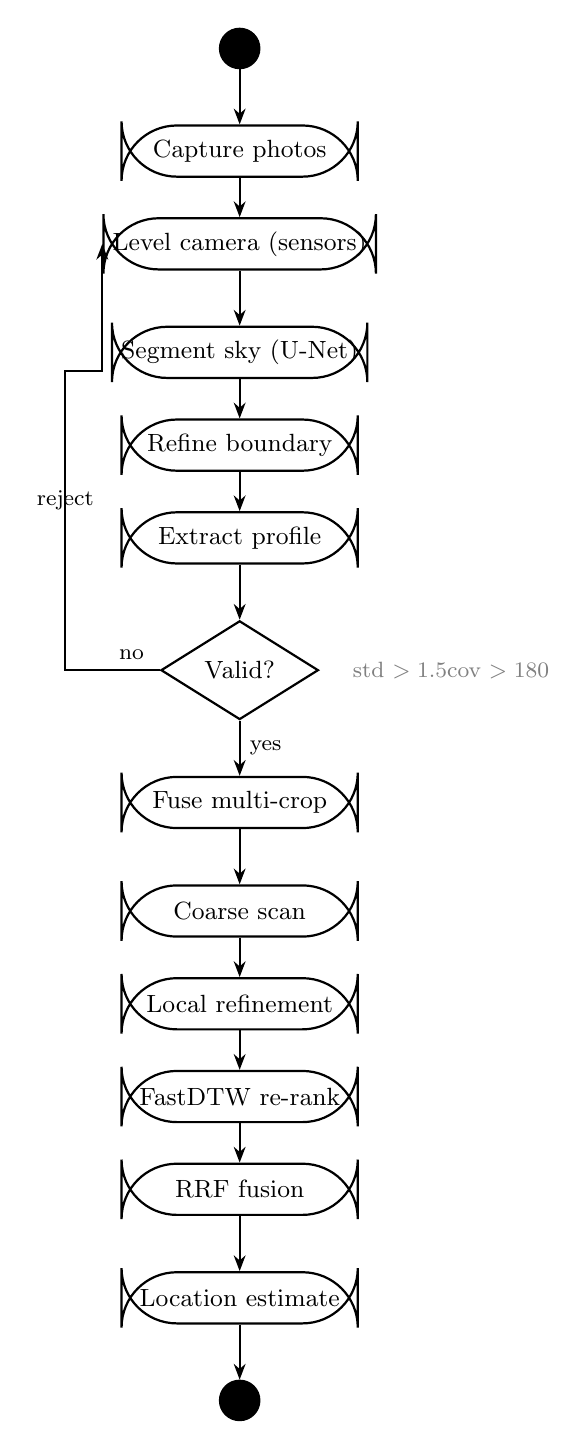
\begin{tikzpicture}[
    node distance=0.6cm and 1.2cm,
    activity/.style={rectangle, draw=black, thick, minimum width=3.0cm, minimum height=0.65cm,
                     text centered, font=\small, rounded corners=20pt},
    decision/.style={diamond, draw=black, thick, minimum width=2.0cm, minimum height=0.7cm,
                     text centered, font=\small, inner sep=1pt},
    startend/.style={circle, draw=black, thick, minimum size=0.5cm, fill=black},
    arr/.style={-{Stealth[length=2mm]}, thick},
    note/.style={font=\footnotesize, text=gray},
]

% Start
\node[startend] (start) {};

% User actions
\node[activity, below=0.7cm of start] (capture) {Capture photos};
\node[activity, below=0.5cm of capture] (level) {Level camera (sensors)};

% System actions
\node[activity, below=0.7cm of level] (seg) {Segment sky (U-Net)};
\node[activity, below=0.5cm of seg] (refine) {Refine boundary};
\node[activity, below=0.5cm of refine] (extract) {Extract profile};

% Decision
\node[decision, below=0.7cm of extract] (valid) {Valid?};
\node[note, right=0.3cm of valid] {std $> 1.5°$\\cov $> 180°$};

% Fusion
\node[activity, below=0.7cm of valid] (fuse) {Fuse multi-crop};

% Matching stages
\node[activity, below=0.7cm of fuse] (coarse) {Coarse scan};
\node[activity, below=0.5cm of coarse] (refine2) {Local refinement};
\node[activity, below=0.5cm of refine2] (dtw) {FastDTW re-rank};
\node[activity, below=0.5cm of dtw] (rrf) {RRF fusion};

% Output
\node[activity, below=0.7cm of rrf] (result) {Location estimate};

% End
\node[startend, below=0.7cm of result] (end) {};

% Arrows
\draw[arr] (start) -- (capture);
\draw[arr] (capture) -- (level);
\draw[arr] (level) -- (seg);
\draw[arr] (seg) -- (refine);
\draw[arr] (refine) -- (extract);
\draw[arr] (extract) -- (valid);

% Decision branches
\draw[arr] (valid) -- node[right, font=\footnotesize] {yes} (fuse);
\draw[arr] (valid.west) -- ++(-1.2,0) node[above, font=\footnotesize, pos=0.3] {no}
    -- node[above, font=\footnotesize] {reject} ++(0,3.8) -| (level.west);

\draw[arr] (fuse) -- (coarse);
\draw[arr] (coarse) -- (refine2);
\draw[arr] (refine2) -- (dtw);
\draw[arr] (dtw) -- (rrf);
\draw[arr] (rrf) -- (result);
\draw[arr] (result) -- (end);

\end{tikzpicture}
\end{document}
